\documentclass[preview]{standalone}

\usepackage{amsmath}
\usepackage{amssymb}
\usepackage{tikz}
\usepackage{pgfplots}
\usepackage{wrapfig}
\usepackage{stellar}
\usepackage{definitions}
\usepackage{bettelini}

\usetikzlibrary{positioning, arrows.meta}

\begin{document}

\id{revolution-solids-integration}
\genpage

\section{Volume of solid revolutions}

\begin{snippet}{volume-of-solid-revolutions-illustration}
    A solid of revolution is a solid made by rotating about an axis a \function
    on an interval \([a;b]\).

    \begin{minipage}{0.5\textwidth}
        \begin{tikzpicture}[
            scale=0.75,
            declare function={
                func(\x) = 0.1 * (\x - 2) * (\x - 2) * sin(\x r) + 2;
            }
        ]

            \draw[-] (0,0) -- (9,0) node [above] {\(x\)};
            \draw[-] (0,-2) -- (0,6) node [above] {\(y\)};
            \draw[domain=0:9, smooth, variable=\x, blue, thick] plot ({\x}, {func(\x)});
        \end{tikzpicture}
    \end{minipage}
    \begin{minipage}{0.5\textwidth}
        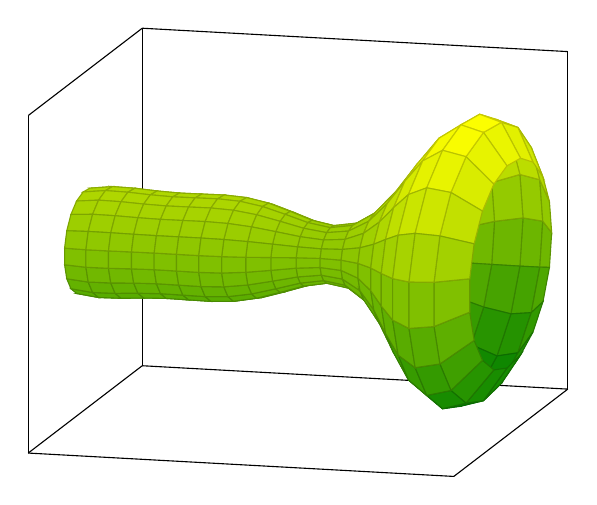
\begin{tikzpicture}[
            declare function={
                func(\x) = 0.1 * (\x - 2) * (\x - 2) * sin(\x r) + 2;
            }
        ]
            \begin{axis}[
                ticks=none,
                colormap/greenyellow,
                view={15}{15}
                ]    
        
                \addplot3[
                    surf,
                    shader=faceted,
                    samples=20,
                    domain=0:9,y domain=0:2*pi,
                    z buffer=sort]
                (x,{func(x) * cos(deg(y))}, {func(x) * sin(deg(y))});
        
            \end{axis}
        \end{tikzpicture}
    \end{minipage}
\end{snippet}

\subsection{Simple revolutions}

\begin{snippet}{simple-revolutions}
Let's start by assuming a rotation aroud the \(x\)-axis of a \function \(y=f(x)\) on \([a;b]\).
we divide the interval into \(n\) subsections of width \(\Delta x = \frac{b-a}{n}\).
For each section we then choose a point \(x^*_k\).
Every subsection is the height of a disk.
The volume is therefore given by the sum of volumes of every disk.
\[
    V \approx \sum_{k=0}^n A(x_k^*) \Delta x
\]
where \(A(x_k^*)\) is the area of the base of the disk of the \(k\)-th subsection. \\
Since we are summing over disks the area of the base is given by
\[
    A=\picircle \cdot {[f(x)]}^2
\]

If we divide the interval into ever smaller sections, the volume becomes exact
\begin{align*}
    V &= \lim_{n\to\infty} \sum_{k=0}^n A(x_k^*) \Delta x
    \\
    &= \integral[a][b][A(x)][x]
\end{align*}

The same approach works for a rotation around the \(y\)-axis.
\[
    V = \integral[a][b][A(y)][y]
\]
where \(A=\picircle \cdot {[f(y)]}^2\)
\end{snippet}

\subsection{Hollow volumes}

\begin{snippet}{hollow-volumes}
When the volume is obtained by rotating an area bounded by two functions, the volume
is partially hollow. This can also happen with a single function.
In this case we can obtain the volume as \(\textbf{outer volume} - \textbf{inner volume}\)
or by summing a set of annuluses rather than disks.
Using annuluses,
\[
    A = \picircle \left[
        {(\text{outer radius})}^2 - {(\text{inner radius})}^2    
    \right]
\]
When we have disks, \(\text{inner radius}=0\). More complex shapes may
require other area functions.
\end{snippet}

\subsection{Other axis}

\begin{snippet}{revolution-integral-other-axis}
When we are rotating a \function about \(x=a\) or \(y=a\)
we need to change the area function accordingly, therefore
usually adjusting the \textbf{outer radius} and \textbf{inner radius}
variables.
\end{snippet}

\subsection{Method of cylinders}

\begin{snippet}{method-of-cylinders}
Sometimes it is tricky or impossible to integrate the volume using disks or annuluses.
We can also cover the volume by using the area of an empty cylinder. In this case we would have
\[
    A = 2\picircle rh
\]
where \(r\) is the radius of the cylinder ad \(h\) is the height of the cylinder.
% https://tutorial.math.lamar.edu/Classes/CalcI/VolumeWithCylinder.aspx
\end{snippet}

\end{document}